%% bare_conf.tex
%% V1.3
%% 2007/01/11
%% by Michael Shell
%% See:
%% http://www.michaelshell.org/
%% for current contact information.
%%
%% This is a skeleton file demonstrating the use of IEEEtran.cls
%% (requires IEEEtran.cls version 1.7 or later) with an IEEE conference paper.
%%
%% Support sites:
%% http://www.michaelshell.org/tex/ieeetran/
%% http://www.ctan.org/tex-archive/macros/latex/contrib/IEEEtran/
%% and
%% http://www.ieee.org/

%%*************************************************************************
%% Legal Notice:
%% This code is offered as-is without any warranty either expressed or
%% implied; without even the implied warranty of MERCHANTABILITY or
%% FITNESS FOR A PARTICULAR PURPOSE! 
%% User assumes all risk.
%% In no event shall IEEE or any contributor to this code be liable for
%% any damages or losses, including, but not limited to, incidental,
%% consequential, or any other damages, resulting from the use or misuse
%% of any information contained here.
%%
%% All comments are the opinions of their respective authors and are not
%% necessarily endorsed by the IEEE.
%%
%% This work is distributed under the LaTeX Project Public License (LPPL)
%% ( http://www.latex-project.org/ ) version 1.3, and may be freely used,
%% distributed and modified. A copy of the LPPL, version 1.3, is included
%% in the base LaTeX documentation of all distributions of LaTeX released
%% 2003/12/01 or later.
%% Retain all contribution notices and credits.
%% ** Modified files should be clearly indicated as such, including  **
%% ** renaming them and changing author support contact information. **
%%
%% File list of work: IEEEtran.cls, IEEEtran_HOWTO.pdf, bare_adv.tex,
%%                    bare_conf.tex, bare_jrnl.tex, bare_jrnl_compsoc.tex
%%*************************************************************************

% *** Authors should verify (and, if needed, correct) their LaTeX system  ***
% *** with the testflow diagnostic prior to trusting their LaTeX platform ***
% *** with production work. IEEE's font choices can trigger bugs that do  ***
% *** not appear when using other class files.                            ***
% The testflow support page is at:
% http://www.michaelshell.org/tex/testflow/



% Note that the a4paper option is mainly intended so that authors in
% countries using A4 can easily print to A4 and see how their papers will
% look in print - the typesetting of the document will not typically be
% affected with changes in paper size (but the bottom and side margins will).
% Use the testflow package mentioned above to verify correct handling of
% both paper sizes by the user's LaTeX system.
%
% Also note that the "draftcls" or "draftclsnofoot", not "draft", option
% should be used if it is desired that the figures are to be displayed in
% draft mode.
%
\documentclass[conference]{IEEEtran}
% Add the compsoc option for Computer Society conferences.
%
% If IEEEtran.cls has not been installed into the LaTeX system files,
% manually specify the path to it like:
% \documentclass[conference]{../sty/IEEEtran}

%%%%%%%%%%%%%%%%%%%%%%%%%%%%%%%%%%%%%%%%%%%%%%%%%%%%%%%%%%%%%%
%%%%%%%%%%%%%%%%%%%%%%%%%%%%%%%%%%%%%%%%%%%%%%%%%%%%%%%%%%%%%%
%%%%%%%%%%%%%%%%%%%%%%   Slavko   %%%%%%%%%%%%%%%%%%%%%%%%%%%%
%%%%%%%%%%%%%%%%%%%%%%%%%%%%%%%%%%%%%%%%%%%%%%%%%%%%%%%%%%%%%%
%%%%%%%%%%%%%%%%%%%%%%%%%%%%%%%%%%%%%%%%%%%%%%%%%%%%%%%%%%%%%%
\usepackage[utf8x]{inputenc}
\usepackage[english]{babel}

%\RequirePackage{geometry}
%\geometry{bindingoffset=0cm, lmargin=2.25cm, rmargin=2.25cm, tmargin=2.25cm, bmargin=2.25cm}

\usepackage{verbatim}
\usepackage{url}
%\usepackage{cases}
\usepackage{algorithm}
\usepackage{multirow}
%\usepackage[cmex10]{amsmath}
\usepackage{alltt}
\usepackage{algorithmic}
\usepackage[dvipsnames,usenames]{color} 

\renewcommand{\algorithmicrequire}{\textbf{Input:}}
\renewcommand{\algorithmicensure}{\textbf{Output:}}

\usepackage{graphicx}
\graphicspath{{../graphics/}}
%\DeclareGraphicsExtensions{.jpg}

\newcommand{\secref}[1]{Section~\ref{#1}}
%\newcommand{\appref}[1]{Appendix~\ref{#1}}
\newcommand{\figref}[1]{Fig.~\ref{#1}}
\newcommand{\tblref}[1]{Table~\ref{#1}}
%\newcommand{\eqref}[1]{Eq.~(\ref{#1})}
\newcommand{\algref}[1]{Algorithm~(\ref{#1})}

\newcommand{\TODO}[0]{{\color{BrickRed}\textbf{TODO}}}
\newcommand{\todo}[1]{{\color{BrickRed}\textbf{TODO:} #1}}
\newcommand{\REDO}[1]{{\color{Mahogany}\textbf{REDO:} \textit{#1}}}
\newcommand{\REFS}[0]{{\color{Sepia}\textbf{REFS}}}
\newcommand{\READ}[1]{{\color{Sepia} #1}}
%%%%%%%%%%%%%%%%%%%%%%%%%%%%%%%%%%%%%%%%%%%%%%%%%%%%%%%%%%%%%%
%%%%%%%%%%%%%%%%%%%%%%%%%%%%%%%%%%%%%%%%%%%%%%%%%%%%%%%%%%%%%%
%%%%%%%%%%%%%%%%%%%%%%%%%%%%%%%%%%%%%%%%%%%%%%%%%%%%%%%%%%%%%%
%%%%%%%%%%%%%%%%%%%%%%%%%%%%%%%%%%%%%%%%%%%%%%%%%%%%%%%%%%%%%%
%%%%%%%%%%%%%%%%%%%%%%%%%%%%%%%%%%%%%%%%%%%%%%%%%%%%%%%%%%%%%%





% Some very useful LaTeX packages include:
% (uncomment the ones you want to load)


% *** MISC UTILITY PACKAGES ***
%
%\usepackage{ifpdf}
% Heiko Oberdiek's ifpdf.sty is very useful if you need conditional
% compilation based on whether the output is pdf or dvi.
% usage:
% \ifpdf
%   % pdf code
% \else
%   % dvi code
% \fi
% The latest version of ifpdf.sty can be obtained from:
% http://www.ctan.org/tex-archive/macros/latex/contrib/oberdiek/
% Also, note that IEEEtran.cls V1.7 and later provides a builtin
% \ifCLASSINFOpdf conditional that works the same way.
% When switching from latex to pdflatex and vice-versa, the compiler may
% have to be run twice to clear warning/error messages.






% *** CITATION PACKAGES ***
%
%\usepackage{cite}
% cite.sty was written by Donald Arseneau
% V1.6 and later of IEEEtran pre-defines the format of the cite.sty package
% \cite{} output to follow that of IEEE. Loading the cite package will
% result in citation numbers being automatically sorted and properly
% "compressed/ranged". e.g., [1], [9], [2], [7], [5], [6] without using
% cite.sty will become [1], [2], [5]--[7], [9] using cite.sty. cite.sty's
% \cite will automatically add leading space, if needed. Use cite.sty's
% noadjust option (cite.sty V3.8 and later) if you want to turn this off.
% cite.sty is already installed on most LaTeX systems. Be sure and use
% version 4.0 (2003-05-27) and later if using hyperref.sty. cite.sty does
% not currently provide for hyperlinked citations.
% The latest version can be obtained at:
% http://www.ctan.org/tex-archive/macros/latex/contrib/cite/
% The documentation is contained in the cite.sty file itself.






% *** GRAPHICS RELATED PACKAGES ***
%
\ifCLASSINFOpdf
  % \usepackage[pdftex]{graphicx}
  % declare the path(s) where your graphic files are
  % \graphicspath{{../pdf/}{../jpeg/}}
  % and their extensions so you won't have to specify these with
  % every instance of \includegraphics
  % \DeclareGraphicsExtensions{.pdf,.jpeg,.png}
\else
  % or other class option (dvipsone, dvipdf, if not using dvips). graphicx
  % will default to the driver specified in the system graphics.cfg if no
  % driver is specified.
  % \usepackage[dvips]{graphicx}
  % declare the path(s) where your graphic files are
  % \graphicspath{{../eps/}}
  % and their extensions so you won't have to specify these with
  % every instance of \includegraphics
  % \DeclareGraphicsExtensions{.eps}
\fi
% graphicx was written by David Carlisle and Sebastian Rahtz. It is
% required if you want graphics, photos, etc. graphicx.sty is already
% installed on most LaTeX systems. The latest version and documentation can
% be obtained at: 
% http://www.ctan.org/tex-archive/macros/latex/required/graphics/
% Another good source of documentation is "Using Imported Graphics in
% LaTeX2e" by Keith Reckdahl which can be found as epslatex.ps or
% epslatex.pdf at: http://www.ctan.org/tex-archive/info/
%
% latex, and pdflatex in dvi mode, support graphics in encapsulated
% postscript (.eps) format. pdflatex in pdf mode supports graphics
% in .pdf, .jpeg, .png and .mps (metapost) formats. Users should ensure
% that all non-photo figures use a vector format (.eps, .pdf, .mps) and
% not a bitmapped formats (.jpeg, .png). IEEE frowns on bitmapped formats
% which can result in "jaggedy"/blurry rendering of lines and letters as
% well as large increases in file sizes.
%
% You can find documentation about the pdfTeX application at:
% http://www.tug.org/applications/pdftex





% *** MATH PACKAGES ***
%
%\usepackage[cmex10]{amsmath}
% A popular package from the American Mathematical Society that provides
% many useful and powerful commands for dealing with mathematics. If using
% it, be sure to load this package with the cmex10 option to ensure that
% only type 1 fonts will utilized at all point sizes. Without this option,
% it is possible that some math symbols, particularly those within
% footnotes, will be rendered in bitmap form which will result in a
% document that can not be IEEE Xplore compliant!
%
% Also, note that the amsmath package sets \interdisplaylinepenalty to 10000
% thus preventing page breaks from occurring within multiline equations. Use:
%\interdisplaylinepenalty=2500
% after loading amsmath to restore such page breaks as IEEEtran.cls normally
% does. amsmath.sty is already installed on most LaTeX systems. The latest
% version and documentation can be obtained at:
% http://www.ctan.org/tex-archive/macros/latex/required/amslatex/math/





% *** SPECIALIZED LIST PACKAGES ***
%
%\usepackage{algorithmic}
% algorithmic.sty was written by Peter Williams and Rogerio Brito.
% This package provides an algorithmic environment fo describing algorithms.
% You can use the algorithmic environment in-text or within a figure
% environment to provide for a floating algorithm. Do NOT use the algorithm
% floating environment provided by algorithm.sty (by the same authors) or
% algorithm2e.sty (by Christophe Fiorio) as IEEE does not use dedicated
% algorithm float types and packages that provide these will not provide
% correct IEEE style captions. The latest version and documentation of
% algorithmic.sty can be obtained at:
% http://www.ctan.org/tex-archive/macros/latex/contrib/algorithms/
% There is also a support site at:
% http://algorithms.berlios.de/index.html
% Also of interest may be the (relatively newer and more customizable)
% algorithmicx.sty package by Szasz Janos:
% http://www.ctan.org/tex-archive/macros/latex/contrib/algorithmicx/




% *** ALIGNMENT PACKAGES ***
%
%\usepackage{array}
% Frank Mittelbach's and David Carlisle's array.sty patches and improves
% the standard LaTeX2e array and tabular environments to provide better
% appearance and additional user controls. As the default LaTeX2e table
% generation code is lacking to the point of almost being broken with
% respect to the quality of the end results, all users are strongly
% advised to use an enhanced (at the very least that provided by array.sty)
% set of table tools. array.sty is already installed on most systems. The
% latest version and documentation can be obtained at:
% http://www.ctan.org/tex-archive/macros/latex/required/tools/


%\usepackage{mdwmath}
%\usepackage{mdwtab}
% Also highly recommended is Mark Wooding's extremely powerful MDW tools,
% especially mdwmath.sty and mdwtab.sty which are used to format equations
% and tables, respectively. The MDWtools set is already installed on most
% LaTeX systems. The lastest version and documentation is available at:
% http://www.ctan.org/tex-archive/macros/latex/contrib/mdwtools/


% IEEEtran contains the IEEEeqnarray family of commands that can be used to
% generate multiline equations as well as matrices, tables, etc., of high
% quality.


%\usepackage{eqparbox}
% Also of notable interest is Scott Pakin's eqparbox package for creating
% (automatically sized) equal width boxes - aka "natural width parboxes".
% Available at:
% http://www.ctan.org/tex-archive/macros/latex/contrib/eqparbox/





% *** SUBFIGURE PACKAGES ***
%\usepackage[tight,footnotesize]{subfigure}
% subfigure.sty was written by Steven Douglas Cochran. This package makes it
% easy to put subfigures in your figures. e.g., "Figure 1a and 1b". For IEEE
% work, it is a good idea to load it with the tight package option to reduce
% the amount of white space around the subfigures. subfigure.sty is already
% installed on most LaTeX systems. The latest version and documentation can
% be obtained at:
% http://www.ctan.org/tex-archive/obsolete/macros/latex/contrib/subfigure/
% subfigure.sty has been superceeded by subfig.sty.



%\usepackage[caption=false]{caption}
%\usepackage[font=footnotesize]{subfig}
% subfig.sty, also written by Steven Douglas Cochran, is the modern
% replacement for subfigure.sty. However, subfig.sty requires and
% automatically loads Axel Sommerfeldt's caption.sty which will override
% IEEEtran.cls handling of captions and this will result in nonIEEE style
% figure/table captions. To prevent this problem, be sure and preload
% caption.sty with its "caption=false" package option. This is will preserve
% IEEEtran.cls handing of captions. Version 1.3 (2005/06/28) and later 
% (recommended due to many improvements over 1.2) of subfig.sty supports
% the caption=false option directly:
%\usepackage[caption=false,font=footnotesize]{subfig}
%
% The latest version and documentation can be obtained at:
% http://www.ctan.org/tex-archive/macros/latex/contrib/subfig/
% The latest version and documentation of caption.sty can be obtained at:
% http://www.ctan.org/tex-archive/macros/latex/contrib/caption/




% *** FLOAT PACKAGES ***
%
%\usepackage{fixltx2e}
% fixltx2e, the successor to the earlier fix2col.sty, was written by
% Frank Mittelbach and David Carlisle. This package corrects a few problems
% in the LaTeX2e kernel, the most notable of which is that in current
% LaTeX2e releases, the ordering of single and double column floats is not
% guaranteed to be preserved. Thus, an unpatched LaTeX2e can allow a
% single column figure to be placed prior to an earlier double column
% figure. The latest version and documentation can be found at:
% http://www.ctan.org/tex-archive/macros/latex/base/



%\usepackage{stfloats}
% stfloats.sty was written by Sigitas Tolusis. This package gives LaTeX2e
% the ability to do double column floats at the bottom of the page as well
% as the top. (e.g., "\begin{figure*}[!b]" is not normally possible in
% LaTeX2e). It also provides a command:
%\fnbelowfloat
% to enable the placement of footnotes below bottom floats (the standard
% LaTeX2e kernel puts them above bottom floats). This is an invasive package
% which rewrites many portions of the LaTeX2e float routines. It may not work
% with other packages that modify the LaTeX2e float routines. The latest
% version and documentation can be obtained at:
% http://www.ctan.org/tex-archive/macros/latex/contrib/sttools/
% Documentation is contained in the stfloats.sty comments as well as in the
% presfull.pdf file. Do not use the stfloats baselinefloat ability as IEEE
% does not allow \baselineskip to stretch. Authors submitting work to the
% IEEE should note that IEEE rarely uses double column equations and
% that authors should try to avoid such use. Do not be tempted to use the
% cuted.sty or midfloat.sty packages (also by Sigitas Tolusis) as IEEE does
% not format its papers in such ways.





% *** PDF, URL AND HYPERLINK PACKAGES ***
%
%\usepackage{url}
% url.sty was written by Donald Arseneau. It provides better support for
% handling and breaking URLs. url.sty is already installed on most LaTeX
% systems. The latest version can be obtained at:
% http://www.ctan.org/tex-archive/macros/latex/contrib/misc/
% Read the url.sty source comments for usage information. Basically,
% \url{my_url_here}.





% *** Do not adjust lengths that control margins, column widths, etc. ***
% *** Do not use packages that alter fonts (such as pslatex).         ***
% There should be no need to do such things with IEEEtran.cls V1.6 and later.
% (Unless specifically asked to do so by the journal or conference you plan
% to submit to, of course. )


% correct bad hyphenation here
\hyphenation{op-tical net-works semi-conduc-tor}


\begin{document}
%
% paper title
% can use linebreaks \\ within to get better formatting as desired
\title{The Role of Semantic Similarity for Intelligent Question Routing}


% author names and affiliations
% use a multiple column layout for up to three different
% affiliations
\author{
\IEEEauthorblockN{Bojan Furlan\IEEEauthorrefmark{1}, Slavko Žitnik\IEEEauthorrefmark{2}\IEEEauthorrefmark{3}, Boško Nikolić\IEEEauthorrefmark{1} and Marko Bajec\IEEEauthorrefmark{2}} 

\IEEEauthorblockA{
\IEEEauthorrefmark{1}University of Belgrade\\
School of Electrical Engineering\\
Bulevar kralja Aleksandra 73\\
RS-11120 Belgrade\\
Email: \{name.surname\}@etf.bg.ac.rs}

\IEEEauthorblockA{
\IEEEauthorrefmark{2}University of Ljubljana\\
Faculty of computer and information science\\
Tržaška cesta 25\\
SI-1000 Ljubljana\\
Email: \{name.surname\}@fri.uni-lj.si}

\IEEEauthorblockA{
\IEEEauthorrefmark{3}Optilab d.o.o.\\
Župančičeva 8\\
SI-5270 Ajdovščina}
}

% conference papers do not typically use \thanks and this command
% is locked out in conference mode. If really needed, such as for
% the acknowledgment of grants, issue a \IEEEoverridecommandlockouts
% after \documentclass

% for over three affiliations, or if they all won't fit within the width
% of the page, use this alternative format:
% 
%\author{\IEEEauthorblockN{Michael Shell\IEEEauthorrefmark{1},
%Homer Simpson\IEEEauthorrefmark{2},
%James Kirk\IEEEauthorrefmark{3}, 
%Montgomery Scott\IEEEauthorrefmark{3} and
%Eldon Tyrell\IEEEauthorrefmark{4}}
%\IEEEauthorblockA{\IEEEauthorrefmark{1}School of Electrical and Computer Engineering\\
%Georgia Institute of Technology,
%Atlanta, Georgia 30332--0250\\ Email: see http://www.michaelshell.org/contact.html}
%\IEEEauthorblockA{\IEEEauthorrefmark{2}Twentieth Century Fox, Springfield, USA\\
%Email: homer@thesimpsons.com}
%\IEEEauthorblockA{\IEEEauthorrefmark{3}Starfleet Academy, San Francisco, California 96678-2391\\
%Telephone: (800) 555--1212, Fax: (888) 555--1212}
%\IEEEauthorblockA{\IEEEauthorrefmark{4}Tyrell Inc., 123 Replicant Street, Los Angeles, California 90210--4321}}




% use for special paper notices
%\IEEEspecialpapernotice{(Invited Paper)}




% make the title area
\maketitle


\begin{abstract}
%\boldmath
Intelligent Question Routing Systems (IQRS) aim to serve as a knowledge exchange medium in an arbitrary field of expertise, where intensive communication between users is required (e.g., large enterprises, e-government agencies, technical support, health care system, army). Other applications can involve a support in educational and collaboration processes, where IQRS facilitates an efficient and effective knowledge exchange between scholars. The benefit coming from deployment of such systems includes: (a) reducing unnecessary “pinging” of experts, which are a valuable resource and (b) increasing the system owners' (enterprise, government, university) quality of service, since users are more satisfied with answers, because their questions are answered by the right persons. In this paper we investigate the role of semantic similarity for each stage of IQRS process. For question analysis we use semantic enrichment, more precisely semantic query expansion with ConceptNet, WordNet (Antelope), and SemNet. Also, for question routing stage we used techniques developed for semantic similarity between two paragraphs sentences.  Finally, for evaluation we used special subsets of Yahoo! L6 Answers dataset from which we extracted three different types of users:  (1) Top questioneers, (2) Top answerers, and (3) Top combination of previous user types to model interest and expertise. Over these users we build special semantic profiles and match them to questions, answers or the whole question threads, according to the specific IQRS stage.
\end{abstract}
% IEEEtran.cls defaults to using nonbold math in the Abstract.
% This preserves the distinction between vectors and scalars. However,
% if the conference you are submitting to favors bold math in the abstract,
% then you can use LaTeX's standard command \boldmath at the very start
% of the abstract to achieve this. Many IEEE journals/conferences frown on
% math in the abstract anyway.

% no keywords




% For peer review papers, you can put extra information on the cover
% page as needed:
% \ifCLASSOPTIONpeerreview
% \begin{center} \bfseries EDICS Category: 3-BBND \end{center}
% \fi
%
% For peerreview papers, this IEEEtran command inserts a page break and
% creates the second title. It will be ignored for other modes.
\IEEEpeerreviewmaketitle



\section{Introduction}
% no \IEEEPARstart
The key functionality of Intelligent Question Routing Systems (IQRS) is that for a question addressed by a user, to provide a good answer by searching the list of all (other) available users. The answer is provided by selecting a certain number of competent users (experts) and forwarding them the question. Selected users can provide an answer, which is then returned to the user that posed the question. The survey of state of the art in IQRS is given in \cite{bib:survey2013} which introduced an original presentation paradigm that generalizes the essence of approaches found in the open literature. The presentation paradigm includes three basic processing stages related to the three major problems of system implementation: question analysis, question forwarding, and users' knowledge profiling. All approaches presented in the survey are analyzed regarding these three basic processing stages. The outcome of the analysis was a proposal for new approaches that tackle identified problems and the work presented in this paper is a consequence of this research.

Questions are usually short in length and even may be ambiguous. Therefore, as a format for acquisition, storing and representation of information related to questions or user profiles, we have chosen an approach in which the detected concepts are presented in the form of concepts cloud (similar to TagCloud visualization) \cite{bib:TAG07, bib:TAG08}. One advantage of this approach is that ``a significant concept has assigned a higher weight,'' which provides an intuitive idea of specific relationships between concepts and their importance in the question. Therefore, the generated concept cloud represents a set of information that describes the question. Concepts together with their weights in this set make the specific context in a broader sense which represents a fingerprint of processed text. This fingerprint is specific to each question and it is similar for questions with the same subject and the same meaning. Finally, this fingerprint reveals specific relationships between questions, and the relationship between the question and the topics which the question touches. On the other hand, for each user IQRS system is maintaining profile which is represented in the same way, describing user’s interests based on his/her questions and answers. Therefore, identified concepts from questions and user profiles are represented as pairs (keyword, weight) which are further referred as evidences.

The task of finding a competent user is done by comparing the information extracted from the question with all available user profiles, giving a ranked list of users or ``candidates to answer''. Based on this ranked list one or more users can be selected, which then should be contacted for an answer. Since the information extracted from the question as well as those maintained in the user profiles are presented in the same way, as lists of evidences, comparison of these two lists is reduced to the calculation of their similarity. Determining the similarity can be carried out by exact comparison, i.e. determining exact matching between words, or by calculating the semantic similarity. Since the question can be semantically very similar to the profile, but still lexically very different, the better results can be achieved by using the semantic similarity. As an example that illustrates this point we can use the appearance of synonyms, words with the identical or very similar meaning, but very different in its form (e.g. words intelligent and smart). Therefore, the main focus of the work presented in this paper is calculation of semantic similarity between the question and the user profile, as well as semantic information extraction from questions and answers in order to calculate this similarity.

The rest of the paper is organized as follows. In \secref{sec:relatedwork} we give a brief overview of related work and available technologies for calculating the semantic similarity of short texts. Next, we introduce our proposed SemSim algorithm for determining the numerical similarity score between the question and the user profile. In \secref{sec:userprofiling} we explain different evidence extraction types and sources that we use. Lastly, we evaluate SemSim on a Yahoo! Answers question and answers dataset and show the results of executions using various settings and in \secref{sec:conclusion}. 
% You must have at least 2 lines in the paragraph with the drop letter
% (should never be an issue)
\TODO drop letter, I wish you the best of success.

\hfill mds
 
\hfill January 11, 2007


% An example of a floating figure using the graphicx package.
% Note that \label must occur AFTER (or within) \caption.
% For figures, \caption should occur after the \includegraphics.
% Note that IEEEtran v1.7 and later has special internal code that
% is designed to preserve the operation of \label within \caption
% even when the captionsoff option is in effect. However, because
% of issues like this, it may be the safest practice to put all your
% \label just after \caption rather than within \caption{}.
%
% Reminder: the "draftcls" or "draftclsnofoot", not "draft", class
% option should be used if it is desired that the figures are to be
% displayed while in draft mode.
%
%\begin{figure}[!t]
%\centering
%\includegraphics[width=2.5in]{myfigure}
% where an .eps filename suffix will be assumed under latex, 
% and a .pdf suffix will be assumed for pdflatex; or what has been declared
% via \DeclareGraphicsExtensions.
%\caption{Simulation Results}
%\label{fig_sim}
%\end{figure}

% Note that IEEE typically puts floats only at the top, even when this
% results in a large percentage of a column being occupied by floats.


% An example of a double column floating figure using two subfigures.
% (The subfig.sty package must be loaded for this to work.)
% The subfigure \label commands are set within each subfloat command, the
% \label for the overall figure must come after \caption.
% \hfil must be used as a separator to get equal spacing.
% The subfigure.sty package works much the same way, except \subfigure is
% used instead of \subfloat.
%
%\begin{figure*}[!t]
%\centerline{\subfloat[Case I]\includegraphics[width=2.5in]{subfigcase1}%
%\label{fig_first_case}}
%\hfil
%\subfloat[Case II]{\includegraphics[width=2.5in]{subfigcase2}%
%\label{fig_second_case}}}
%\caption{Simulation results}
%\label{fig_sim}
%\end{figure*}
%
% Note that often IEEE papers with subfigures do not employ subfigure
% captions (using the optional argument to \subfloat), but instead will
% reference/describe all of them (a), (b), etc., within the main caption.


% An example of a floating table. Note that, for IEEE style tables, the 
% \caption command should come BEFORE the table. Table text will default to
% \footnotesize as IEEE normally uses this smaller font for tables.
% The \label must come after \caption as always.
%
%\begin{table}[!t]
%% increase table row spacing, adjust to taste
%\renewcommand{\arraystretch}{1.3}
% if using array.sty, it might be a good idea to tweak the value of
% \extrarowheight as needed to properly center the text within the cells
%\caption{An Example of a Table}
%\label{table_example}
%\centering
%% Some packages, such as MDW tools, offer better commands for making tables
%% than the plain LaTeX2e tabular which is used here.
%\begin{tabular}{|c||c|}
%\hline
%One & Two\\
%\hline
%Three & Four\\
%\hline
%\end{tabular}
%\end{table}


% Note that IEEE does not put floats in the very first column - or typically
% anywhere on the first page for that matter. Also, in-text middle ("here")
% positioning is not used. Most IEEE journals/conferences use top floats
% exclusively. Note that, LaTeX2e, unlike IEEE journals/conferences, places
% footnotes above bottom floats. This can be corrected via the \fnbelowfloat
% command of the stfloats package.


\section{Related Work \& Available Technologies}
\label{sec:relatedwork}
Based on the analysis of existing approaches for semantic similarity of short texts (or short text semantic similarity - STSS) it was concluded that none of the available solutions can be directly applied for determining the similarity between questions and user profiles. Therefore, determining the similarity is done by using a bag-of-words approach based on a modification of LinSTSS approach \cite{bib:LinSTSS}, in which for all evidences in the question $Q$ we find the most similar matching evidences in the profile $P$. We decided to base our approach on LinSTSS for the following reasons:
\begin{enumerate}
	\item This approach includes weights assigned to each compared word, i.e. can naturally deal with evidences.
	\item It does not rely on any external knowledge base (e.g. WordNet), manually created inference rules or specific linguistic tools, which would be an obstacle in working with languages that lack these resources. Furthermore, the LinSTSS approach does not use the semantic similarity measure alone, but includes string similarity measure as well, so it gives better results for different forms of infrequent proper nouns, which is one of the major shortcomings of the knowledge-based approaches \cite{bib:JITA}.
	\item Finally, LinSTSS is inspired by the method proposed in \cite{bib:1} that relies on a similar bag-of-words approach, but uses word specificity as in \cite{bib:2} to weight the word similarity. However it overcomes the problem of method \cite{bib:2}, which has a tendency to overestimate text similarity because it allows multiple words from one text to be paired up with a single word in the other text.
\end{enumerate}	
The last item is significant in determining the semantic similarity of two short texts, since it is important to determine which pairs of sentences are semantically similar, but also which are different. However, we wanted to explore if this stands also for the task of finding competent users, i.e. calculating similarity between the question and the user profile, because in this case it is necessary to determine just which profile is the most similar to the question, while it is not necessary to determine those that are different. To some extent this relates to one-class-classification problem, since we only have positive examples, e.g. we are aware of the user that provided the best answer to the question, but negative examples are unknown, i.e. we don’t know which users are not able to provide the best answer. Therefore, we introduced modification named SemSim to determine the highest (maximum) similarity between evidences from the question to evidences from the profile, but not vice versa.

The rest of the section gives a brief description of algorithms and tools that are used for user profiling, i.e. analyzing questions and answers. To be able to measure similarity between questions and user profiles, we had to extract as many semantic evidences about users as possible, their behaviour as possible. In this study we used the following techniques and sources:
\begin{itemize}
	\item {\bf ConceptNet}~\cite{bib:conceptnet} is a semantic knowledge base that describes general human knowledge. It includes words and common phrases from many written texts. They are related through open domain predicates and through common knowledge. The database was created manually and partially automatically from Wiktionary and ReVerb system, which is an open information extraction tool that extracts binary relationships of type {\it phrase-relation-phrase} in an unsupervised manner. The whole database contains 414 thousand English concepts and 903 thousand relationships between them.
	\item {\bf Antelope} (Advanced Natural Language Object-oriented Processing Environement)~\cite{bib:antelope} is a natural language processing framework (NLP) that can handle large corpora and consists of many extensible modular components. It uses an extended lexicon version of WordNet lexicon with improved conceptualization and integrates a higher level formal ontology. The main components offer syntactic and semantic analysis of texts, anaphora extraction, word sense disambiguation and paraphrase extraction. It also includes access to other opensource NLP libraries such as Stanford Parser, WordNet and VerbNet.
	\item {\bf SemNet} (Semantic Network of Terms)~\cite{bib:semnet} is a large-scale network of technical terminology which allows querying terms and retrieving ranked lists of their semantically related terms. The network was automatically constructed based on the noun terms from English Google Books Ngram Dataset using word co-occurrence analysis. The network consists of 2.8 million distinct single and multi-word terms and 37.5 million weighted edges between them. SemNet includes a large part of the same concepts and relationships from similar semantic knowledge bases such as WordNet~\cite{bib:wordnet} and ConceptNet~\cite{bib:conceptnet}. 
	\item {\bf TF-IDF} (term frequency-inverse document frequency) is a general numerical statistic that defines the importance of each word in a document collection. It is often used in information retrieval and text mining as it gives good string-based performance. 
\end{itemize}
	
\section{Semantic Similarity}
\label{sec:alg}
This section describes phase-by-phase the algorithm of determining the numerical similarity score between the question and the user profile, followed by an example of the execution. 
	
1. {\it Preprocessing} begins with the text cleaning procedure which deletes all text characters not belonging to the native script of the language in question, removes numbers and words that contain numbers, eliminates punctuation marks, removes stopwords, shifts all capital letters into lower caseand finally, lemmatizes them. Processing then continues with the removal of stop words from the given texts and the remaining words from both texts are then stemmed. After this stage, if there are evidences where their keyword consists of more than one word, for each word is created new evidence with the same weight as the original one, e.g. from evidence (botanical gardens, 0.5) two evidences are created (botanical, 0.5) and (gardens, 0.5). If there are multiple evidences with the same keyword they are merged into one by calculating resulting weight with the probabilistic T-conorm: 
\begin{equation}
	\label{eq:tconorm}
	{\rm sum(a,b)}\;=\;a+b-a\cdot b
\end{equation}

After the preprocessing input data, the question is represented with a array $Q$ given in \ref{eq:q} and the profile $P$ is given in \ref{eq:p}. $Q$ consists of pairs $(q_i,w(q_i))$ representing evidences, where $q_i$ is the keyword and $w(q_i)$ is its assigned weight. Similarly, $P$ is consisted of pairs $(u_i,w(u_i))$. The length of array $Q$ is $m$ and for $P$ is $n$.
\begin{equation}
	\label{eq:q}
	Q = \{(q_1,w(q_1)),(q_2,w(q_2)),\ldots(q_m,w(q_m))\}
\end{equation} 

\begin{equation}
	\label{eq:p}
	U=\{(u_1,w(u_1)),(u_2,w(u_2)),\ldots(u_n,w(u_n))\}
\end{equation}

    
2. {\it Processing of keywords appearing in both question and profile} starts with the identification of those words which are then removed from further processing. Their similarity scores are equal to 1, so their final weight is equal to normalized weight $w(q_i,u_i)$, which is calculated using $w(q_i)$ and $w(u_j)$ as follows:
\begin{equation}
	\label{eq:w}
	w(q_i,u_j)=2^{w(q_i)\cdot w(u_j)-1}
\end{equation}

After calculating their values, we add them up into a similarity sum $S_{same}$, and then discard these words from further consideration. For MaxSim this step is omitted since we want to determine the highest (maximum) similarity, as it will be explained in step 7.

3. {\it String similarity matrix construction} creates a matrix $M_1$ with dimensions $m\times n$ in which every cell is occupied by a numerical value $\alpha$, which lies between 0 and 1 representing the string similarity between the column-word and the row-word. The rows of the matrix are used for the remaining words from the question, while the columns represent the remaining words from the profile. A zero value denotes entirely different string contents, while a value of one indicates a perfect string match. The approach which we used to calculate string similarity is the same as in \cite{bib:LinSTSS}.

\begin{equation}
	\label{eq:m1}
	M_1 = 
\left( 
	\begin{array}{ccc}
		\alpha_{11} & \cdots & \alpha_{1n} \\
		\vdots & \ddots & \vdots \\
		\alpha_{m1} & \cdots & \alpha_{mn} 
	\end{array} 
\right)
\end{equation}

4. {\it Semantic similarity matrix construction} creates a matrix $M_2$ with dimensions $m\times n$ in which every cell is occupied by a numerical value $\beta$ which lies between 0 and 1 representing the semantic similarity between the column-word and the row-word. The rows of the matrix are used for the words from the question, while the columns represent the words from the profile. Similar to the string similarity measurement, a zero value denotes entirely different semantic contents, while a value of one indicates a perfect semantic match. We gain the semantic similarity of words in a pair by calculating the cosine similarity in the same way as in \cite{bib:LinSTSS}.

\begin{equation}
	\label{eq:m2}
	M_2 = 
\left( 
	\begin{array}{ccc}
		\beta_{11} & \cdots & \beta_{1n} \\
		\vdots & \ddots & \vdots \\
		\beta_{m1} & \cdots & \beta_{mn} 
	\end{array} 
\right)
\end{equation}


5. {\it Similarity matrix unification} combines the string and the semantic similarity matrices into one by multiplying their values by a certain ponderation factor and adding them up as in \ref{eq:m3a}. We used ponderation values of 0.45 and 0.55 for the string and semantic similarity scores, respectively.

\begin{eqnarray}
	\label{eq:m3a}
	M_3 & = & \psi M_1 + \varphi M_2 \\
	1 & = & \psi + \varphi
\end{eqnarray}

\begin{equation}
	\label{eq:m3b}
	M_3 = 
\left( 
	\begin{array}{ccc}
		\gamma_{11} & \cdots & \gamma_{1n} \\
		\vdots & \ddots & \vdots \\
		\gamma_{m1} & \cdots & \gamma_{mn} 
	\end{array} 
\right)
\end{equation}

6. The {\it weighted matrix construction} begins with the creation of a normalized weighted matrix in which every cell is occupied by a weight $w(q_i,u_j)$ calculated using \ref{eq:w}. The final similarity matrix $M_4$, shown in \ref{eq:m4}, is gained by multiplying each cell of the unified similarity matrix with the corresponding value $\gamma_{i,j}$ from $M_3$.

\begin{equation}
	\label{eq:m4}
	M_4 = 
\left( 
	\begin{array}{ccc}
		w(q_1,u_1)\cdot \gamma_{11} & \cdots & w(q_1,u_n)\cdot \gamma_{1n} \\
		\vdots & \ddots & \vdots \\
		w(q_m,u_1)\cdot \gamma_{m1} & \cdots & w(q_m,u_n)\cdot \gamma_{mn} 
	\end{array} 
\right)
\end{equation}

7. {\it Best word pair selections} start with the final similarity matrix. The goal is to match words according to their mutual similarity score. Hence, we search for the highest value within the final similarity matrix, and add it to a similarity sum $S_{different}$. We then remove the row and the column of the matrix to which the selected cell belonged, thereby discarding all other word pairs in which words from the chosen pair appeared. We repeat this procedure until there are no more rows and/or columns left in the matrix.
 
For MaxSim approach this step is executed differently since we wanted to determine the highest (maximum) similarity between evidences from question to profile, but not vice versa. Therefore, only for each row, which represents words from the question, we search for the highest value within the final similarity matrix, and add it to a similarity sum $S_{different}$. Since in the step 2 none of the words is omitted for this approach, $S_{same}=0$.
 
8. The {\it final similarity score calculation} is performed by utilizing the following formula:
 
 \begin{equation}
	\label{eq:s}
	S(Q,U) = \frac{(S_{same}+S_{different})\times (m+n)}{2mn}
\end{equation}
	
	\TODO include link to the software repository
	\TODO example:
	

	
\begin{table}[!t]
\renewcommand{\arraystretch}{1.3}
	\caption{String similarity matrix - ConceptExtractor}
	\label{tab:stringsim}
	\centering
	\begin{tabular}{l||c|c|c|c}\hline
	&\bfseries meatbal & \bfseries spagetti & \bfseries good & \bfseries recipi \\\hline\hline
		\bfseries chemistry & 0.03 & 0.02 & 0.00 & 0.03\\
		\bfseries shrimp & 0.02 & 0.04 & 0.00 & 0.09\\
		\bfseries ocean & 0.08 & 0.02 & 0.03 & 0.02\\
		\bfseries lake & 0.02 & 0.05 & 0.00 & 0.03\\
		\bfseries river & 0.02 & 0.02 & 0.00 & 0.07\\
	\hline
	\end{tabular}
\end{table}

\begin{table}[!t]
\renewcommand{\arraystretch}{1.3}
	\caption{Semantic similarity matrix - ConceptExtractor}
	\label{tab:semsimm}
	\centering
	\begin{tabular}{l||c|c|c|c}\hline
	&\bfseries meatbal & \bfseries spagetti & \bfseries good & \bfseries recipi \\\hline\hline
		\bfseries chemistry & 0.00 & 0.00 & 0.00 & 0.00\\
		\bfseries shrimp & 0.00 & 0.00 & 0.10 & 0.03\\
		\bfseries ocean & 0.00 & 0.00 & 0.08 & 0.05\\
		\bfseries lake & 0.00 & 0.00 & 0.08 & 0.05\\
		\bfseries river & 0.00 & 0.00 & 0.06 & 0.05\\
	\hline
	\end{tabular}
\end{table}

\begin{table}[!t]
\renewcommand{\arraystretch}{1.3}
	\caption{Term similarity matrix - ConceptExtractor}
	\label{tab:termsim}
	\centering
	\begin{tabular}{l||c|c|c|c}\hline
	&\bfseries meatbal & \bfseries spagetti & \bfseries good & \bfseries recipi \\\hline\hline
		\bfseries chemistry & 1.00 & 1.00 & 0.33 & 0.30\\
		\bfseries shrimp & 0.85 & 0.85 & 0.28 & 0.25\\
		\bfseries ocean & 0.92 & 0.92 & 0.30 & 0.28\\
		\bfseries lake & 0.90 & 0.90 & 0.30 & 0.27\\
		\bfseries river & 1.00 & 1.00 & 0.33 & 0.30\\
	\hline
	\end{tabular}
\end{table}

\begin{table}[!t]
\renewcommand{\arraystretch}{1.3}
	\caption{Joint similarity matrix - ConceptExtractor}
	\label{tab:jointsim}
	\centering
	\begin{tabular}{l||c|c|c|c}\hline
	&\bfseries meatbal & \bfseries spagetti & \bfseries good & \bfseries recipi \\\hline\hline
		\bfseries chemistry & 0.01 & 0.01 & 0.00 & 0.01\\
		\bfseries shrimp & 0.01 & 0.02 & 0.03 & 0.03\\
		\bfseries ocean & 0.03 & 0.01 & 0.04 & 0.02\\
		\bfseries lake & 0.01 & 0.02 & 0.03 & 0.02\\
		\bfseries river & 0.01 & 0.01 & 0.02 & 0.04\\
	\hline
	\end{tabular}
\end{table}
	
\section{User Profiling}
\label{sec:userprofiling}
There are many approaches to extract information from textual documents. The advantages of statistical approaches are mostly higher precision on large corpora, easier implementation and longer history of research. On the other hand, if we need to process a short text, methods from the field of computational linguistics will give the best results. In order to build efficient user profiles, we collect a number of evidences from user's posts. Each evidence is a tuple...\TODO We separate evidences by source, which can origin from question body, answer body, question title, whole post thread or IQRS system. The more detailed description of data set that we used is given in next section.  

Before the evidence extraction we first employ some preprocessing techniques. This step is carried the same way as in step 1 of the proposed algorithm (\secref{sec:alg}). From these we further extract evidences of the following types:

{\bf Concept extractor}:
In our implementation of concept extractor we integrated Antelope and ConceptNet (\secref{sec:relatedwork}). Since the Antelope tool is based on a much smaller but more precise WordNet lexicon, it is designed to recognize named entities (e.g., names of people, organizations, states and cities) with high precision, but with limited number of concepts. Together with integrated context extraction it can contribute to better identify concepts. On the other hand, ConceptNet contains much richer semantic network, which provides better results in identifying existing and related concepts, but it does not support named entity recognition or context extraction. When we combined these tools (Antelope and ConceptNet) during the query expansion, we got better results than using them individually.

Since both tools, in addition to the identified concepts, determine the weight of the extracted concept within the range $(0,1]$, we use the following approach to combine both values: If only one of the tools finds some concept, it retains the weight, otherwise we calculate the resulting weight using the probabilistic T-conorm (\ref{eq:tconorm}). 

In order to obtain better results and reduce the number of incorrectly identified concepts we also use the following rules:
\begin{enumerate}
	\item We empirically defined linear relationship between the minimum weight of a concept (i.e., threshold) and a length of the text:
$$
	{\rm min(weight)} = 0.875 + {\rm \#words\_in\_text} \cdot 0.125
$$
If the weight of a concept is less than the minimum weight, it is removed and therefore not used in further calculations.
	\item Since it is much harder to detect the topic from the long text rather than from the short text, which consists only of important concepts, the process of context identification is carried as follows: (1) We first detect all the concepts using Antelope and ConceptNet. (2) Then we again use Antelope to find context for all the concepts from the previous step, considering higher precision.
\end{enumerate}

{\bf SemNet} allows for searching ranked lists of semantically related terms. For each extracted word in the preprocessing step we select three most semantically related terms as SemNet evidences. For example, the word ``car'' is within SemNet described with the following evidences: (``front'', 0.038), (``side'', 0.024) and (``truck'', 0.024).

{\bf TF-IDF} is a standard measure for weighting words within text documents. Intuitively the word has different weight depending on the source of occurence. Therefore we calculate TF-IDF measures separately for question titles, question bodies and answers. For example, a word ``car'' has the following TF-IDF weights\footnote{The example was taken calculated on the post 1512658 from the L6 dataset.}: (1) 0.163 in the question title, (2) 0.066 in the question body, (3) and 0.0246 in the best answer. 

{\bf Categories}:
Each post also contains associated categories. In our dataset there are three hierarchical category types. Their values are more thoroughly explained within the dataset description (\secref{sec:dataset}).


\section{Evaluation}
\TODO write section intro


\subsection{Dataset}
\label{sec:dataset}
We reviewed many question answering (QA) systems and datasets. Finally, we decided to use Yahoo! Answers Webscope L6 dataset~\cite{bib:yahool6} because it contains a broad range of distinct question categories and there are enough active users in each of the categories that we selected. Other datasets could be extracted from sites such as AskVille (\url{http://askville.amazon.com}), Mahalo (\url{http://mahalo.com}), Quora (\url{http://quora.com}) and StackOverflow (\url{http://stackoverflow.com}). The latter also includes a lot of users but it does not have specified specific categories and more importantly, the whole dataset is mostly single domain oriented. Furthermore, there are lots of other systems like AllExperts (\url{http://allexperts.com}), Ask.com (\url{http://ask.com}), Answers.com (\url{http://answers.com}) and others that lack of one or more public features to build useful dataset.

Yahoo! Answers is a QA site where people post questions and answers, which are publicly available to any web user. The L6 dataset was collected from this site in 2007 and it includes all the questions (i.e. 4483032) and their corresponding answers. Next to these data some anonymized metadata is included, so that we can can extract evidences related to the each user.

Questions and answers represent instances of post type and one question with its all available answers forms a thread. Each post instance consists of text in the body, selection of main category, category and subcategory and the id of the user who wrote the post. Questions additionally contain also title. For answer posts, the owner user is known only if it was considered as the best answer for the question, which imposed the limitation that only for the user that provided the best answer we can relate extracted evidences.

User instances are completely anonymized, so we modeled them using their id. Also, we counted how many answers or questions the users posted in specific category type.

From the full dataset we extracted three database types:
\begin{itemize}
	\item {\bf Type 1}: This dataset models interest as it contains users that asked at least ten questions and each of these questions must have at least five answers.
	\item {\bf Type 2}: To model knowledge, we extracted users who best answered at least ten questions. Again, each question thread needed to have at least five answers.
	\item {\bf Type 3}: To jointly represent interest and knowledge, we extracted users that asked at least five questions and best answered at least five questions. Also, each of these threads needed to have at least five answers.
\end{itemize}
Each dataset type contains 100 users which are distinct across the datasets. As there are many different categories in the data, we representatively selected five of them and extracted 100 users for each dataset. Distribution of users per each categoriy is shown \tblref{tab:datasets}.

\begin{table}[!h]
	\centering
	\renewcommand{\arraystretch}{1.3}
	\caption{Distribution of post categories in each database type}
	\label{tab:datasets}
	\begin{tabular}{l|c}\hline
		Category & Number of selected users\\\hline\hline
		Society \& Culture & 35\\
		Food \& Drink & 35\\
		Computers \& Internet & 15\\
		Travel & 10\\
		Cars \& Transportation & 5\\\hline\hline
		Total & 100\\\hline
	\end{tabular}
\end{table}

\subsection{Results and Discussion}
To evaluate our work we use metrics mean reciprocal rank (MRR) and Precision@N (P@N) which are widely used in the field. They are defined as follows: (1) MRR is a measure to evaluate information retrieval task in which a list of possible responses to a query is ordered by a probability of correctness. The score is defined as the average of the reciprocal ranks for a set of queries $Q$,
$$
	{\rm MRR = }\frac{1}{|Q|}\sum_{i=1}^{|Q|}\frac{1}{rank_i}.
$$
(2) Precision is the fraction of the documents retrieved that are relevant to a query. P@N is therefore precision which is evaluated at a given cut-off rank $N$ (i.e. considering only top $N$ results). In our domain it measures the proportion of correctly selected experts among all experts or intuitively a probability of how likely asking among the top $N$ experts will result in getting a correct answer.
\TODO


	
\begin{table*}[!h]
	\centering
	\renewcommand{\arraystretch}{1.3}
	\caption{Achieved MRR scores on all DB Types with all settings}
	\label{tab:resultsmrr}
	\begin{tabular}{l||ccc}\hline
	
		\multicolumn{4}{l}{DB Type 1 - Question evidences}\\\hline\hline
		& Unweighted & Weighted & Max Sem Sim\\
		CE, SN, TFIDF & 0.11 & 0.14 & 0.05\\
		CE & 0.15 & 0.16 & 0.10\\
		Cat1 & 0.20 & 0.20 & 0.18\\
		Cat2 & 0.07 & 0.07 & 0.07\\
		Cat3 & 0.13 & 0.13 & 0.12\\
		Cat1,2,3 & 0.21 & 0.21 & 0.15\\
		Cat1, CE & 0.18 & 0.17 & 0.12\\
		Cat1,2,3, CE & 0.20 & 0.22 & 0.15\\
		TFIDF & 0.15 & 0.05 & 0.05\\
		TFIDF, SN & 0.11 & 0.06 & 0.05\\
		SN & 0.08 & 0.08 & 0.06\\
		\hline
		
		\multicolumn{4}{l}{DB Type 2 - Answer evidences}\\\hline\hline
		& Unweighted & Weighted & Max Sem Sim\\
		CE, SN, TFIDF & 0.14 & 0.13 & 0.05\\
		CE & 0.15 & 0.16 & 0.07\\
		Cat1,2,3 & 0.22 & 0.22 & 0.15\\
		CE, Cat1,2,3 & 0.17 & 0.19 & 0.09\\
		TFIDF & 0.18 & 0.05 & 0.05\\
		SN, TFIDF & 0.16 & 0.05 & 0.05\\
		\hline
		
		\multicolumn{4}{l}{DB Type 2 - Thread evidences}\\\hline\hline
		& Unweighted & Weighted & Max Sem Sim\\
		CE & 0.15 & 0.17 & 0.04\\
		SN & 0.07 & 0.07 & 0.06\\
		CE, SN, TFIDF & 0.16 & 0.04 & 0.04\\
		Cat1,2,3 & 0.21 & 0.21 & 0.03\\
		TFIDF & 0.18 & 0.05 & 0.04\\
		SN, TFIDF & 0.15 & 0.04 & 0.04\\
		\hline
		
		\multicolumn{4}{l}{DB Type 3 - Answer evidences}\\\hline\hline
		& Unweighted & Weighted & Max Sem Sim\\
		CE, SN, TFIDF & 0.11 & 0.06 & 0.06\\
		CE & 0.10 & 0.10 & 0.05\\
		Cat1,2,3 & 0.18 & 0.18 & 0.16\\
		CE, Cat1,2,3 & 0.16 & 0.20 & 0.09\\
		TFIDF & 0.10 & 0.06 & 0.05\\
		SN, TFIDF & 0.11 & 0.06 & 0.05\\
		SN & 0.09 & 0.10 & 0.06\\
		\hline
		
		\multicolumn{4}{l}{DB Type 3 - Thread evidences}\\\hline\hline
		& Unweighted & Weighted & Max Sem Sim\\
		CE, SN, TFIDF & 0.14 & 0.04 & 0.04\\
		CE & 0.11 & 0.11 & 0.03\\
		Cat1,2,3 & 0.17 & 0.17 & 0.16\\
		CE, Cat1,2,3 & 0.16 & 0.21 & 0.04\\
		TFIDF & 0.16 & 0.04 & 0.04\\
		SN, TFIDF & 0.13 & 0.04 & 0.04\\
		SN & 0.09 & 0.11 & 0.06\\
		\hline
		
	\end{tabular}
\end{table*}

\begin{table*}[!h]
	\centering
	\renewcommand{\arraystretch}{1.3}
	\caption{Achieved P@N scores on all DB Types with all settings}
	\label{tab:resultsmrr}
	\begin{tabular}{l||l|ccccc}\hline
	
		\multicolumn{7}{l}{DB Type 1 - Question evidences}\\\hline\hline
		& N & 5 & 10 & 15 & 20 & 30\\\hline
		
		\multirow{3}{*}{CE, SN, TFIDF} & Unweighted & 0.13 & 0.27 & 0.34 & 0.45 & 0.56\\
		 & Weighted & 0.13 & 0.28 & 0.36 & 0.46 & 0.57\\
		 & MaxSemSim & 0.05 & 0.11 & 0.2 & 0.27 & 0.38\\
		 
		\multirow{3}{*}{CE} & Unweighted & 0.16 & 0.25 & 0.39 & 0.46 & 0.63\\
		 & Weighted & 0.19 & 0.27 & 0.38 & 0.45 & 0.62\\
		 & MaxSemSim & 0.12 & 0.19 & 0.25 & 0.31 & 0.43\\ 
		\hline
		
		\multirow{3}{*}{Cat1} & Unweighted & 0.23 & 0.33 & 0.51 & 0.61 & 0.72\\
		 & Weighted & 0.23 & 0.33 & 0.51 & 0.61 & 0.72\\
		 & MaxSemSim & 0.22 & 0.32 & 0.44 & 0.53 & 0.74\\ 
		\hline
		
		\multirow{3}{*}{Cat2} & Unweighted & 0.05 & 0.1 & 0.3 & 0.44 & 0.69\\
		 & Weighted & 0.05 & 0.1 & 0.3 & 0.44 & 0.69\\
		 & MaxSemSim & 0.05 & 0.1 & 0.3 & 0.44 & 0.69\\ 
		\hline
		
		\multirow{3}{*}{Cat3} & Unweighted & 0.2 & 0.27 & 0.35 & 0.43 & 0.68\\
		 & Weighted & 0.2 & 0.27 & 0.35 & 0.43 & 0.68\\
		 & MaxSemSim & 0.17 & 0.24 & 0.35 & 0.48 & 0.62\\ 
		\hline
		
		\multirow{3}{*}{Cat1,2,3} & Unweighted & 0.29 & 0.44 & 0.55 & 0.61 & 0.8\\
		 & Weighted & 0.29 & 0.44 & 0.55 & 0.61 & 0.8\\
		 & MaxSemSim & 0.19 & 0.35 & 0.41 & 0.52 & 0.74\\ 
		\hline
		
		\multirow{3}{*}{Cat1, CE} & Unweighted & 0.21 & 0.36 & 0.47 & 0.55 & 0.66\\
		 & Weighted & 0.24 & 0.36 & 0.47 & 0.54 & 0.66\\
		 & MaxSemSim & 0.15 & 0.23 & 0.3 & 0.37 & 0.5\\ 
		\hline
		
		\multirow{3}{*}{Cat1,2,3, CE} & Unweighted & 0.24 & 0.4 & 0.58 & 0.62 & 0.7\\
		 & Weighted & 0.29 & 0.46 & 0.59 & 0.64 & 0.74\\
		 & MaxSemSim & 0.17 & 0.3 & 0.42 & 0.52 & 0.63\\ 
		\hline
		
		\multirow{3}{*}{TFIDF} & Unweighted & 0.21 & 0.27 & 0.4 & 0.51 & 0.65\\
		 & Weighted & 0.06 & 0.09 & 0.15 & 0.21 & 0.33\\
		 & MaxSemSim & 0.06 & 0.09 & 0.15 & 0.2 & 0.33\\ 
		\hline
		
		\multirow{3}{*}{TFIDF, SN} & Unweighted & 0.13 & 0.24 & 0.32 & 0.41 & 0.55\\
		 & Weighted & 0.06 & 0.09 & 0.16 & 0.2 & 0.37\\
		 & MaxSemSim & 0.06 & 0.09 & 0.15 & 0.19 & 0.3\\ 
		\hline
		
		\multirow{3}{*}{SN} & Unweighted & 0.1 & 0.16 & 0.25 & 0.3 & 0.38\\
		 & Weighted & 0.1 & 0.16 & 0.27 & 0.3 & 0.38\\
		 & MaxSemSim & 0.04 & 0.11 & 0.17 & 0.24 & 0.34\\ 
		\hline		

		\multicolumn{7}{l}{DB Type 2 - Answer evidences}\\\hline\hline
		& N & 5 & 10 & 15 & 20 & 30\\\hline
		\hline
		
		\multirow{3}{*}{CE, SN, TFIDF} & Unweighted & 0.21 & 0.3 & 0.39 & 0.46 & 0.57\\
		 & Weighted & 0.2 & 0.29 & 0.39 & 0.45 & 0.57\\
		 & MaxSemSim & 0.03 & 0.09 & 0.13 & 0.18 & 0.28\\ 
		\hline
		
		\multirow{3}{*}{CE} & Unweighted & 0.21 & 0.28 & 0.32 & 0.36 & 0.48\\
		 & Weighted & 0.2 & 0.28 & 0.31 & 0.35 & 0.47\\
		 & MaxSemSim & 0.07 & 0.15 & 0.2 & 0.24 & 0.35\\ 
		\hline
		
		\multirow{3}{*}{Cat1,2,3} & Unweighted & 0.33 & 0.48 & 0.59 & 0.69 & 0.87\\
		 & Weighted & 0.33 & 0.48 & 0.59 & 0.69 & 0.87\\
		 & MaxSemSim & 0.27 & 0.39 & 0.54 & 0.63 & 0.79\\ 
		\hline
		
		\multirow{3}{*}{CE, Cat1,2,3} & Unweighted & 0.24 & 0.35 & 0.5 & 0.56 & 0.7\\
		 & Weighted & 0.27 & 0.41 & 0.49 & 0.63 & 0.7\\
		 & MaxSemSim & 0.09 & 0.25 & 0.37 & 0.47 & 0.49\\ 
		\hline
		
		\multirow{3}{*}{TFIDF} & Unweighted & 0.25 & 0.32 & 0.43 & 0.48 & 0.62\\
		 & Weighted & 0.04 & 0.09 & 0.14 & 0.16 & 0.31\\
		 & MaxSemSim & 0.04 & 0.09 & 0.13 & 0.18 & 0.28\\ 
		\hline
		
		\multirow{3}{*}{SN, TFIDF} & Unweighted & 0.23 & 0.31 & 0.41 & 0.52 & 0.63\\
		 & Weighted & 0.04 & 0.09 & 0.14 & 0.2 & 0.32\\
		 & MaxSemSim & 0.04 & 0.09 & 0.15 & 0.17 & 0.26\\ 
		\hline		
	\end{tabular}
\end{table*}		
		
\begin{table*}[!h]
	\centering
	\renewcommand{\arraystretch}{1.3}
	\caption{Achieved P@N scores on all DB Types with all settings}
	\label{tab:resultsmrr}
	\begin{tabular}{l||l|ccccc}\hline		
		
		\multicolumn{7}{l}{DB Type 2 - Thread evidences}\\\hline\hline
		& N & 5 & 10 & 15 & 20 & 30\\\hline
		\hline
		
		\multirow{3}{*}{CE} & Unweighted & 0.22 & 0.26 & 0.34 & 0.42 & 0.56\\
		 & Weighted & 0.2 & 0.27 & 0.36 & 0.46 & 0.63\\
		 & MaxSemSim & 0.01 & 0.04 & 0.08 & 0.1 & 0.18\\ 
		\hline
		
		\multirow{3}{*}{SN} & Unweighted & 0.09 & 0.18 & 0.26 & 0.33 & 0.41\\
		 & Weighted & 0.06 & 0.18 & 0.26 & 0.33 & 0.41\\
		 & MaxSemSim & 0.05 & 0.11 & 0.17 & 0.21 & 0.29\\ 
		\hline
		
		\multirow{3}{*}{CE, SN, TFIDF} & Unweighted & 0.19 & 0.29 & 0.46 & 0.55 & 0.71\\
		 & Weighted & 0.02 & 0.06 & 0.1 & 0.14 & 0.19\\
		 & MaxSemSim & 0.02 & 0.06 & 0.09 & 0.15 & 0.19\\ 
		\hline
		
		\multirow{3}{*}{Cat1,2,3} & Unweighted & 0.31 & 0.48 & 0.60 & 0.70 & 0.87\\
		 & Weighted & 0.31 & 0.48 & 0.60 & 0.70 & 0.87\\
		 & MaxSemSim & 0.01 & 0.04 & 0.11 & 0.17 & 0.29\\ 
		\hline
		
		\multirow{3}{*}{TFIDF} & Unweighted & 0.21 & 0.33 & 0.46 & 0.57 & 0.74\\
		 & Weighted & 0.04 & 0.08 & 0.13 & 0.18 & 0.22\\
		 & MaxSemSim & 0.04 & 0.08 & 0.12 & 0.18 & 0.22\\ 
		\hline
		
		\multirow{3}{*}{SN, TFIDF} & Unweighted & 0.16 & 0.31 & 0.49 & 0.56 & 0.73\\
		 & Weighted & 0.04 & 0.07 & 0.09 & 0.13 & 0.17\\
		 & MaxSemSim & 0.04 & 0.07 & 0.1 & 0.13 & 0.16\\ 
		\hline		
		
		\multicolumn{7}{l}{DB Type 3 - Answer evidences}\\\hline\hline
		& N & 5 & 10 & 15 & 20 & 30\\\hline
		\hline
		
		\multirow{3}{*}{CE, SN, TFIDF} & Unweighted & 0.14 & 0.23 & 0.27 & 0.32 & 0.49\\
		 & Weighted & 0.05 & 0.14 & 0.18 & 0.34 & 0.45\\
		 & MaxSemSim & 0.07 & 0.13 & 0.17 & 0.22 & 0.31\\ 
		\hline
		
		\multirow{3}{*}{CE} & Unweighted & 0.14 & 0.2 & 0.27 & 0.35 & 0.46\\
		 & Weighted & 0.12 & 0.2 & 0.25 & 0.34 & 0.48\\
		 & MaxSemSim & 0.04 & 0.1 & 0.15 & 0.2 & 0.32\\ 
		\hline
		
		\multirow{3}{*}{Cat1,2,3} & Unweighted & 0.22 & 0.41 & 0.54 & 0.66 & 0.81\\
		 & Weighted & 0.22 & 0.41 & 0.54 & 0.66 & 0.81\\
		 & MaxSemSim & 0.2 & 0.37 & 0.45 & 0.55 & 0.76\\ 
		\hline
		
		\multirow{3}{*}{CE, Cat1,2,3} & Unweighted & 0.23 & 0.39 & 0.5 & 0.55 & 0.64\\
		 & Weighted & 0.33 & 0.41 & 0.51 & 0.59 & 0.65\\
		 & MaxSemSim & 0.13 & 0.27 & 0.35 & 0.41 & 0.55\\ 
		\hline
		
		\multirow{3}{*}{TFIDF} & Unweighted & 0.15 & 0.29 & 0.35 & 0.45 & 0.59\\
		 & Weighted & 0.04 & 0.1 & 0.15 & 0.22 & 0.4\\
		 & MaxSemSim & 0.04 & 0.13 & 0.16 & 0.25 & 0.32\\ 
		\hline
		
		\multirow{3}{*}{SN, TFIDF} & Unweighted & 0.15 & 0.24 & 0.31 & 0.39 & 0.51\\
		 & Weighted & 0.04 & 0.11 & 0.18 & 0.29 & 0.44\\
		 & MaxSemSim & 0.05 & 0.12 & 0.18 & 0.23 & 0.32\\ 
		\hline
		
		\multirow{3}{*}{SN} & Unweighted & 0.14 & 0.18 & 0.28 & 0.34 & 0.41\\
		 & Weighted & 0.14 & 0.18 & 0.28 & 0.33 & 0.42\\
		 & MaxSemSim & 0.09 & 0.11 & 0.15 & 0.22 & 0.32\\ 
		\hline		
		
		\multicolumn{7}{l}{DB Type 3 - Thread evidences}\\\hline\hline
		& N & 5 & 10 & 15 & 20 & 30\\\hline
		\hline
		
		\multirow{3}{*}{CE, SN, TFIDF} & Unweighted & 0.23 & 0.35 & 0.46 & 0.55 & 0.63\\
		 & Weighted & 0.04 & 0.06 & 0.11 & 0.18 & 0.27\\
		 & MaxSemSim & 0.03 & 0.05 & 0.11 & 0.15 & 0.26\\ 
		\hline
		
		\multirow{3}{*}{CE} & Unweighted & 0.12 & 0.26 & 0.33 & 0.42 & 0.57\\
		 & Weighted & 0.14 & 0.26 & 0.37 & 0.43 & 0.55\\
		 & MaxSemSim & 0.02 & 0.05 & 0.06 & 0.09 & 0.23\\ 
		\hline
		
		\multirow{3}{*}{Cat1,2,3} & Unweighted & 0.22 & 0.39 & 0.54 & 0.61 & 0.75\\
		 & Weighted & 0.22 & 0.39 & 0.54 & 0.61 & 0.75\\
		 & MaxSemSim & 0.17 & 0.33 & 0.43 & 0.55 & 0.72\\ 
		\hline
		
		\multirow{3}{*}{CE, Cat1,2,3} & Unweighted & 0.18 & 0.34 & 0.45 & 0.56 & 0.76\\
		 & Weighted & 0.25 & 0.48 & 0.63 & 0.65 & 0.83\\
		 & MaxSemSim & 0.01 & 0.04 & 0.07 & 0.11 & 0.3\\ 
		\hline
		
		\multirow{3}{*}{TFIDF} & Unweighted & 0.21 & 0.3 & 0.41 & 0.49 & 0.68\\
		 & Weighted & 0.04 & 0.08 & 0.12 & 0.18 & 0.28\\
		 & MaxSemSim & 0.04 & 0.08 & 0.12 & 0.18 & 0.27\\ 
		\hline
		
		\multirow{3}{*}{SN, TFIDF} & Unweighted & 0.18 & 0.32 & 0.41 & 0.52 & 0.65\\
		 & Weighted & 0.04 & 0.06 & 0.11 & 0.18 & 0.22\\
		 & MaxSemSim & 0.04 & 0.06 & 0.11 & 0.17 & 0.24\\ 
		\hline
		
		\multirow{3}{*}{SN} & Unweighted & 0.14 & 0.21 & 0.33 & 0.41 & 0.49\\
		 & Weighted & 0.17 & 0.25 & 0.32 & 0.43 & 0.49\\
		 & MaxSemSim & 0.07 & 0.08 & 0.17 & 0.22 & 0.28\\ 
		\hline				
	\end{tabular}
\end{table*}
	
\begin{figure}[!t]
	\centering
	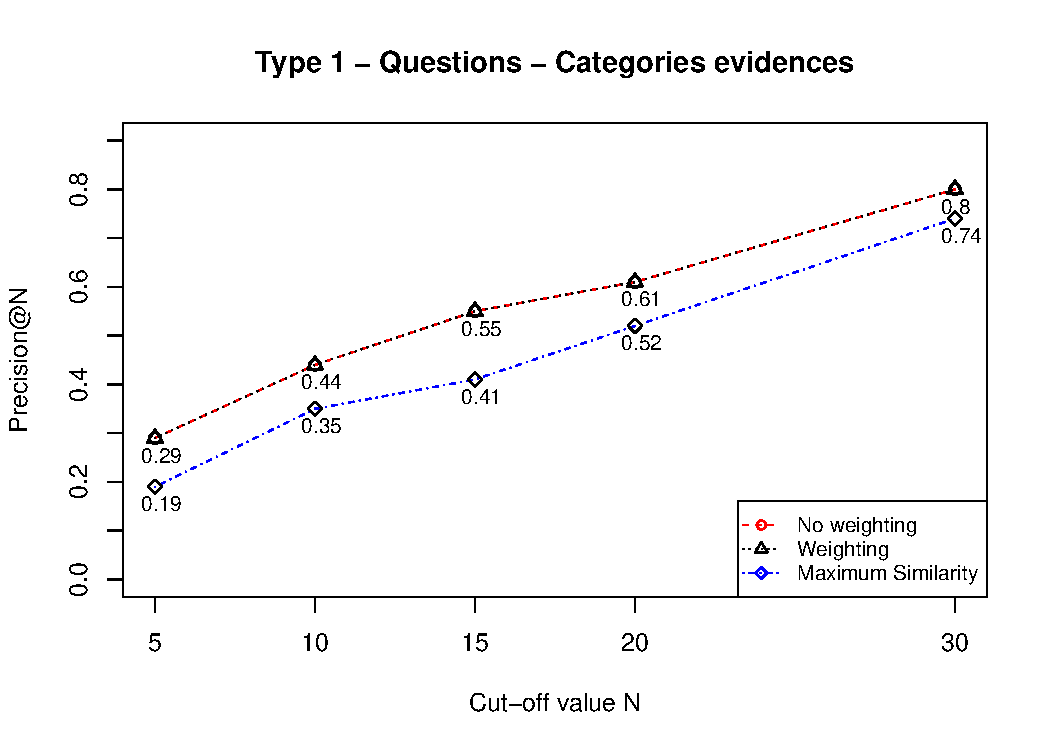
\includegraphics[width=3.3in]{type1questions_PAtN.pdf}
	\caption{Precision @ N results for database type 1 using questions and categories evidences.}
	\label{fig:pntype1}
\end{figure}

\begin{figure}[!t]
	\centering
	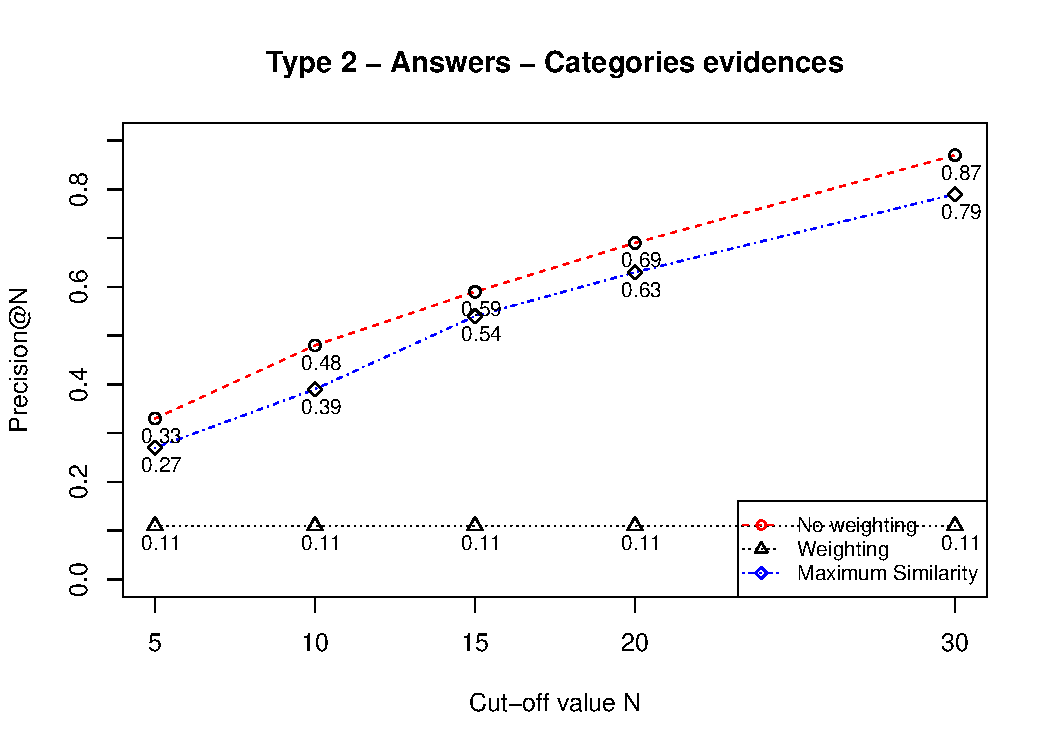
\includegraphics[width=3.3in]{type2answers_PAtN.pdf}
	\caption{Precision @ N results for database type 2 using answers and categories evidences.}
	\label{fig:pntype2}
\end{figure}

\begin{figure}[!t]
	\centering
	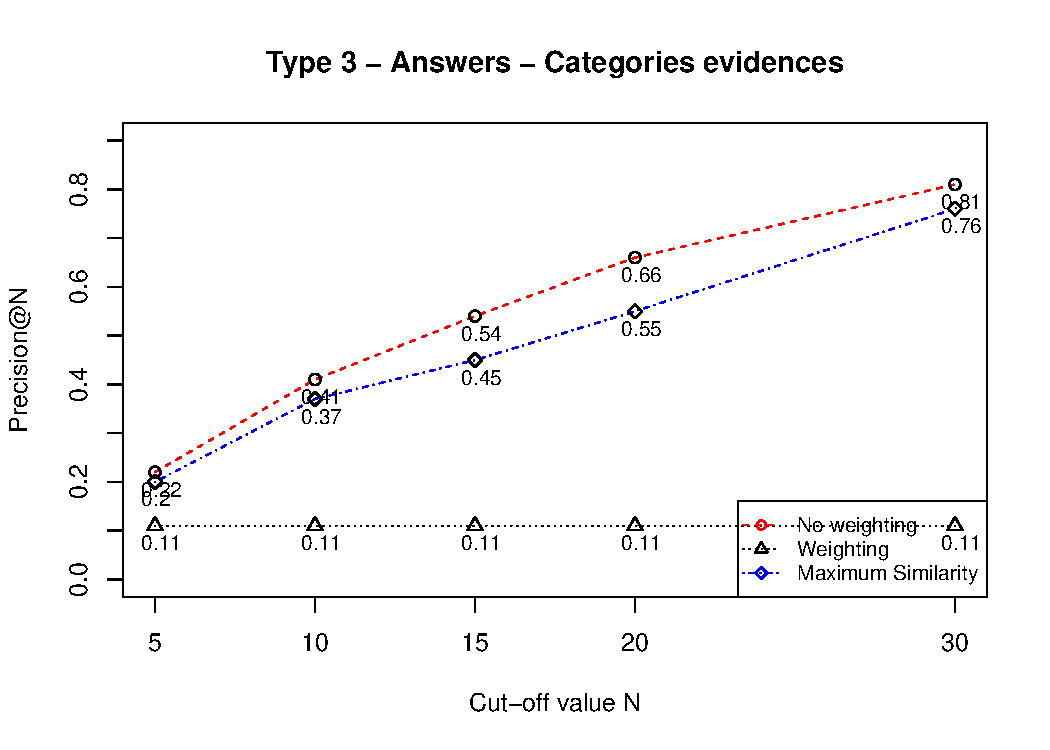
\includegraphics[width=3.3in]{type3answers_PAtN.pdf}
	\caption{Precision @ N results for database type 3 using answers and categories evidences.}
	\label{fig:pntype3}
\end{figure}


\begin{figure*}[!t]
	\centering
	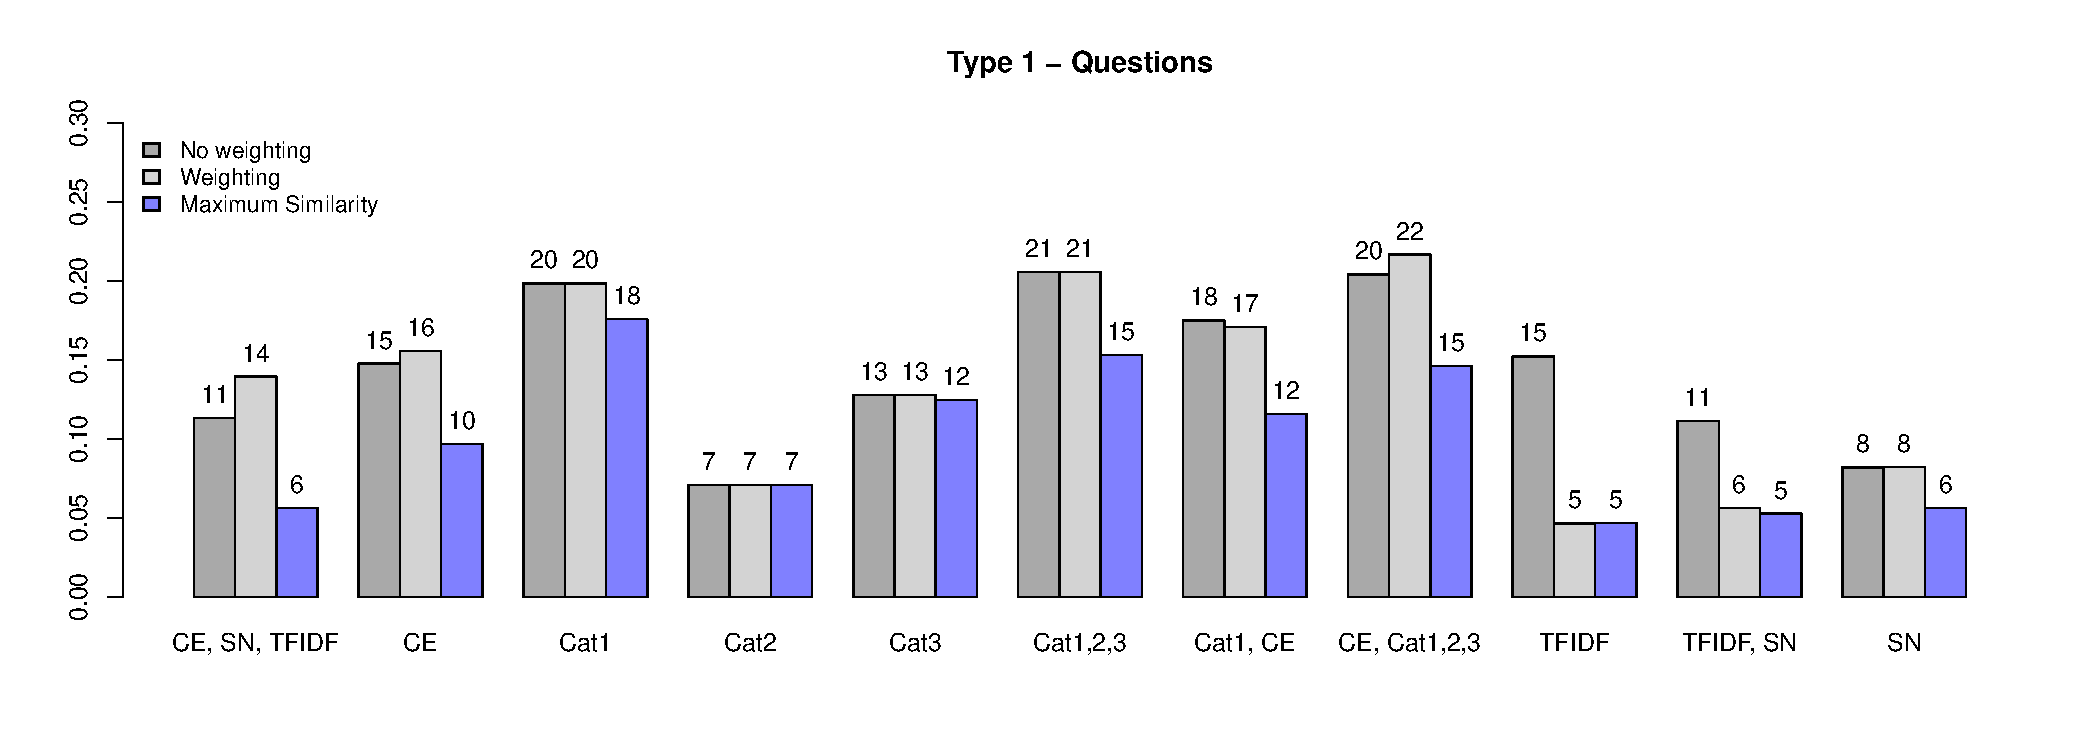
\includegraphics[width=\textwidth]{mrrType1Questions.pdf}
	\caption{Mean reciprocal rank scores for database of type 1 on questions evidences.}
	\label{fig:mrrtype1}
\end{figure*}

\begin{figure*}[!t]
	\centering
	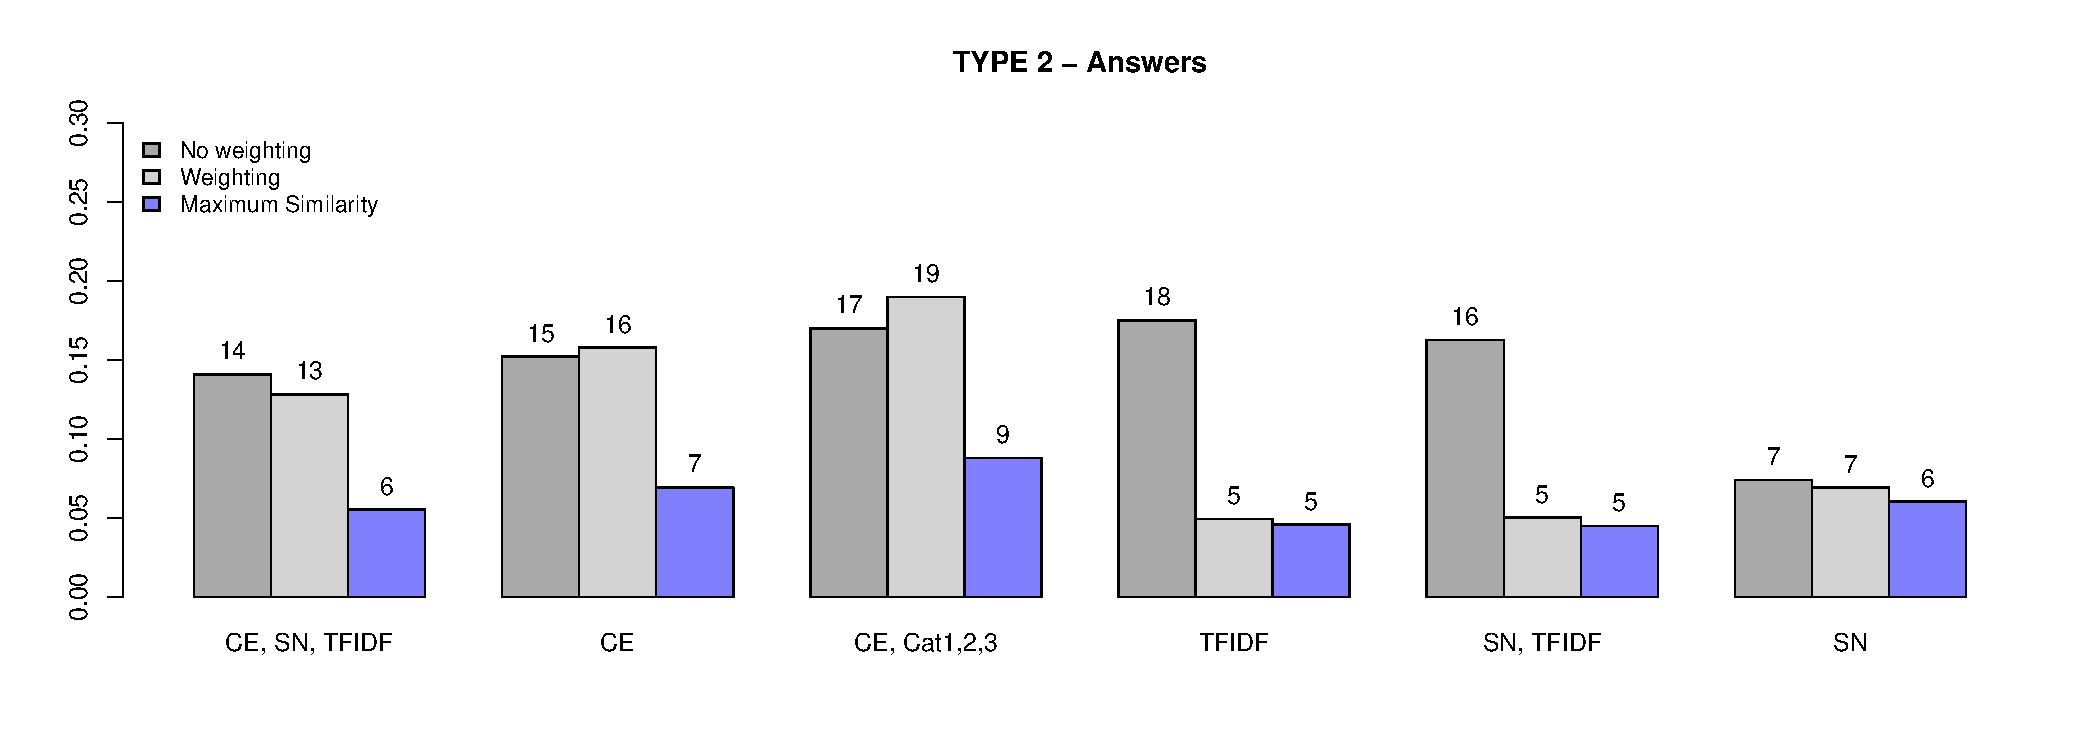
\includegraphics[width=\textwidth]{mrrType2Answers.pdf}
	\caption{Mean reciprocal rank scores for database of type 2 on answers evidences.}
	\label{fig:mrrtype2}
\end{figure*}

\begin{figure*}[!t]
	\centering
	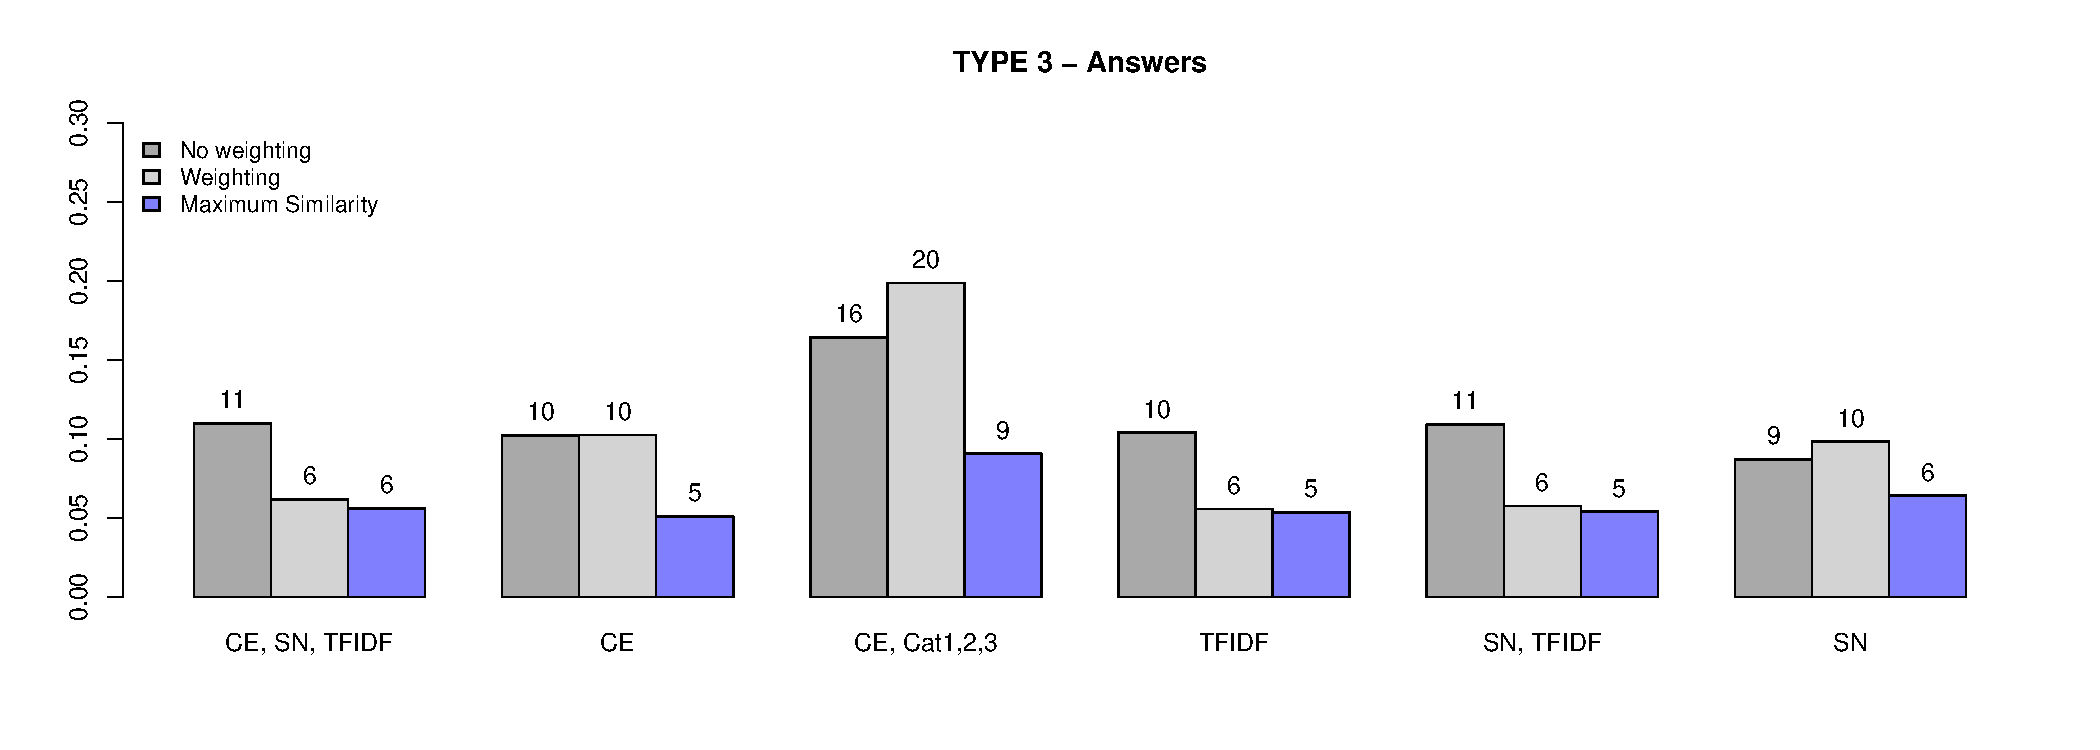
\includegraphics[width=\textwidth]{mrrType3Answers.pdf}
	\caption{Mean reciprocal rank scores for database of type 3 on answers evidences.}
	\label{fig:mrrtype3}
\end{figure*}

\begin{figure*}[!t]
	\centering
	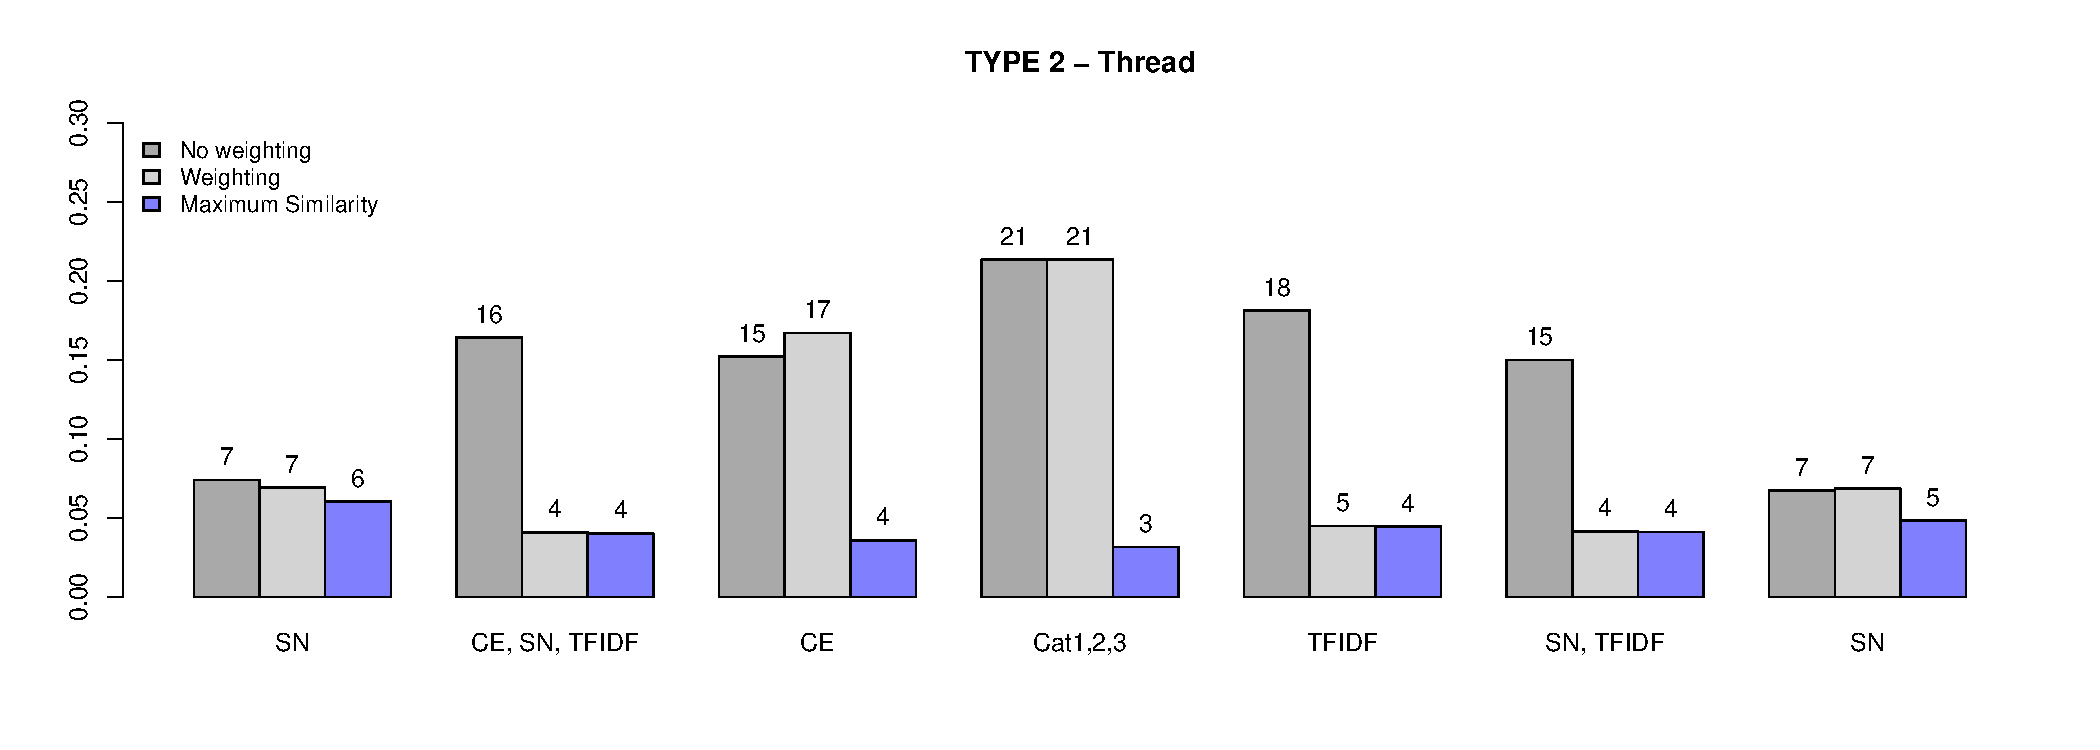
\includegraphics[width=\textwidth]{mrrType2Thread.pdf}
	\caption{Mean reciprocal rank scores for database of type 2 on thread evidences.}
	\label{fig:mrrtype3}
\end{figure*}

\begin{figure*}[!t]
	\centering
	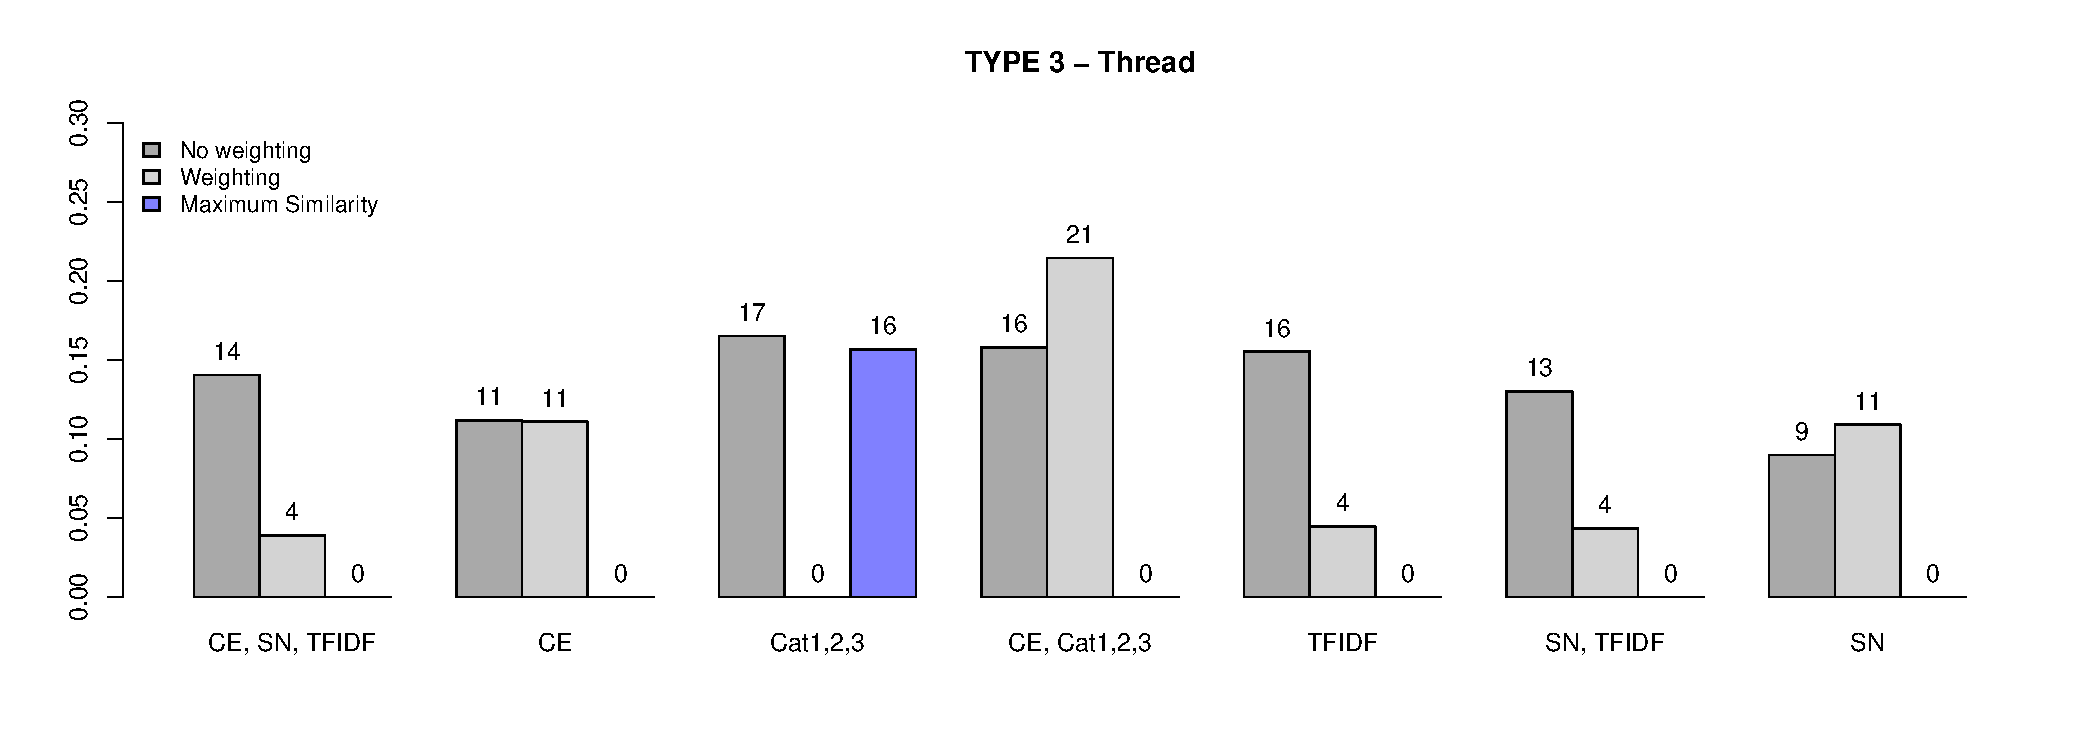
\includegraphics[width=\textwidth]{mrrType3Thread.pdf}
	\caption{Mean reciprocal rank scores for database of type 3 on thread evidences.}
	\label{fig:mrrtype3}
\end{figure*}

\section{Conclusion}
\label{sec:conclusion}
The conclusion goes here.




% conference papers do not normally have an appendix


% use section* for acknowledgement
\section*{Acknowledgment}
The work has been supported by the Slovene Research Agency ARRS within the research program P2-0359 and part financed by the European Union, European Social Fund. It was also partially funded by the Ministry of Education and Science of the Republic of Serbia (projects III44009, 44006, 32047).





% trigger a \newpage just before the given reference
% number - used to balance the columns on the last page
% adjust value as needed - may need to be readjusted if
% the document is modified later
%\IEEEtriggeratref{8}
% The "triggered" command can be changed if desired:
%\IEEEtriggercmd{\enlargethispage{-5in}}

% references section

% can use a bibliography generated by BibTeX as a .bbl file
% BibTeX documentation can be easily obtained at:
% http://www.ctan.org/tex-archive/biblio/bibtex/contrib/doc/
% The IEEEtran BibTeX style support page is at:
% http://www.michaelshell.org/tex/ieeetran/bibtex/
\bibliographystyle{IEEEtran}
% argument is your BibTeX string definitions and bibliography database(s)
\bibliography{IEEEabrv,informatics2013}
%
% <OR> manually copy in the resultant .bbl file
% set second argument of \begin to the number of references
% (used to reserve space for the reference number labels box)


%\begin{thebibliography}{1}
%\bibitem{IEEEhowto:kopka}
%H.~Kopka and P.~W. Daly, \emph{A Guide to \LaTeX}, 3rd~ed.\hskip 1em plus
%  0.5em minus 0.4em\relax Harlow, England: Addison-Wesley, 1999.
%\end{thebibliography}




% that's all folks
\end{document}


